\chapter{Framework} \label{chapter:framework}
Point cloud cleaning is an intensive interactive task. Improved segmentation techniques can therefore not be created without considering the user interface that facilitates them. A bad interface can negate any gains to be had from better tools. An interface that is effective and easy to use is therefore a prerequisite for a faster segmentation process.

In \autoref{ch:background} it was argued that in order for a user to be effective, i.e. achieve a predetermined level of accuracy, techniques with a small area of influence are required in addition to techniques with large areas of influence. For example, a polygon selection tool can select a large area but can lack accuracy. In order to achieve a good level of accuracy a brush tool that has a small area of influence is needed to correct mislabeled points within the larger selection achieved by the lasso tool. It is clear that proprietary systems provide a larger range of tools when compared to open source alternatives. Proprietary tools also tend to be more user friendly. It would thus be preferable to use a proprietary system as a base for testing new segmentation techniques. Unfortunately, due to their closed sourced nature, we are forced to either extend an open source system or create one.

Allowing a user to undo an action or return to a previous state is an important usability heuristic \cite{Nielsen2005}. The importance of undo to user productivity was reiterated in informal talks with users of Meshlab in the heritage domain. Adding undo functionality to Meshlab or Cloud Compare is not a trivial task as the inclusion on such a feature would require updates to many extensions and plug-ins.

Meshlab and Cloud Compare are also not specifically designed for segmentation tasks. Meshlab lacks the concept of layers. As a result, intermediate segmentations cannot be saved for later refinement. To perform a cleaning task, points have to be irreversibly deleted. Cloud compare is more suitable for segmentation tasks as it lets one move subsets of points into a new cloud that can be edited independently. Segmentation tools are however limited to a polygon select tool.

There is a small number of existing segmentation tools in open source systems and they have hard to fix usability problems. It therefore appears that there is little to be gained, without significant effort, from using Meshlab or Cloud Compare as a foundation for new segmentation tools. It was therefore decided to create a new open source system designed specifically for range image segmentation. A fresh start allows us to reproduce the best parts from existing systems in order to create solid foundation for new tools.

To reiterate, the goal of our system is to create an extensible open source framework for point cloud segmentation because existing system do not meet our needs.

\begin{itemize}
\item{Manage segmentations}
\item{Visualize data}
\item{Extensible via plug-ins}
\item{Cross platform}
\item{Easy to use}
\end{itemize}

The following sections provide design and implementation details our core system. The core system does not include segmentation tools. These will be discussed separately in later chapters.

\todo{Explicit summary of what was argued: ie  base on what as argued, list of requirements, maybe do this below}

\section{Architecture}

In order to maximize extensibility, our system is designed around a plug-in architecture. It consists of a core of common functionality and a set of plug-ins (see \autoref{fig:system}). Plug-in architectures fall on a spectrum based on the amount of functionality present in the core. Some systems, like QTCreator, only have a plug-in manager and basic GUI in the core while everything else is a plug-in. In others the core contains most of the functionality and plug-ins only add to it.

Meshlab falls somewhere in the middle. It provides a core that includes a viewer, a camera model and other basic functionality. Meshlab lets one load four types of plug-ins. \emph{Edit} plug-ins lets one manipulate a model interactively, \emph{filters} manipulate a model in a non-interactive manner, \emph{IO} plug-ins let one import and export files, and \emph{render} plug-ins affects how the model is rendered. Each plug-in implements an interface that the plug-manager uses to initialise the plug-in in a predetermined way. This limits the type of functionality a plug-in can implement to that provided by the four predetermined types.

In our system we follow a similar approach. The viewer and camera model are part of the core. Plug-ins however implement a single interface in contrast with Meshlab's 4 types. Control is inverted in that the plug-in manager lets the plug-in hook itself into the system which allows it to implement any functionality. This approach is more flexible as plug-in functionality does not have fit a predetermined class. Dependencies between plug-ins can also be specified. Before the plug-in manager loads and initializes modules, a dependency graph is constructed to determined the loading order. The plug-in manager monitors a predetermined directory for changes. If a new plug-in is found it will be loaded at runtime. Deleted plug-ins are also dynamically unloaded and updated plug-ins are reload. Dynamic loading of plug-ins in this way has the benefit of reducing development as the entire system does not need to be restarted when components change.

\section{Core}

\begin{figure}[ht]
  \centering
  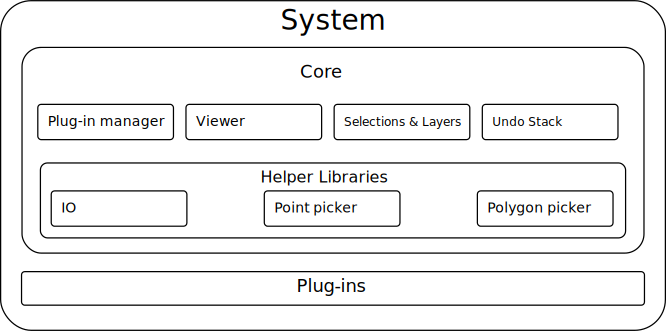
\includegraphics[width=.75\linewidth]{images/system}
  \caption[System architecture]{The system is implemented as a plug-in architecture. The user interface and state management is handled by the core system. Segmentation and other tools that manipulate the system state are loaded into the system as plug-ins.}
  \label{fig:system}
\end{figure}

\todo{Explain what is going on in captions}
\todo{Have algorithms everywhere}
\todo{System boot up in an algorithm}

\todo{Explain dependency graph and meta data}
\todo{Cross platform is useful for the comunity ast large, mention it as, plugins and compilation steps are non trivial, however that is not the main focus, provid emore detail in apendix, because it is peripheral}

The system core implements the functionality needed to view range images, manage range images, keep track of segmentations and load plug-ins. Some additional functionality that could be moved to plug-ins are also resident in the core system. This includes basic file import and helper functions for common UI problems.

\subsection{IO}

The system is currently limited to dealing with range images that with 3D coordinates and intensity values. Importing Cyclone PTX range images is built into of core system. PTX is an ASCII based interchange format created by Leica. The file format may contain multiple range images with 3D coordinates, intensity and RGB values. The file header also contains a 4x4 matrix that represents the registration transformation in addition to the scan grid dimensions \cite{Leica}. Following the header is the point data arranged in ordered in column major order. The format contains all the scan data including non returned points as that are represented as 0 0 0 for the XYZ coordinate.

Because a large number of points are typically not returned, they are discarded when loading a PTX file into the system. This reduces memory consumption and simplifies 3D rendering and manipulation. A separate data structure is kept that maps returned points back to their position in the scan grid. This insures that operations that rely on a point's position in the original scan grid, such as 2d rendering and normal computation, can still be performed. It also means that the PTX file can be saved in its original format.

The system makes use of PCL (Point Cloud Library) \cite{Rusu2011} data structures. This allows us to use many popular point cloud algorithms without implementing them from scratch.

\subsection{Segments} \label{sec:segments}

The core system need to keep track subsets of points identified by segmentation plug-ins. The data structures used in this book keeping task require some careful consideration. Our review of tools in existing systems allow us to gather some requirements.

Interactive tools such as a lasso or brush tool require that points be added or removed from a selection real time. Representing a selection as an array of indices would require an $O(n)$ operation for adding or removing points. If we instead represent a selection as an array of boolean values that are mapped to points, a selection can be modified in constant time. This representation however has the disadvantage of only allowing binary segmentations. One way of overcoming this limitation is to create additional boolean arrays for new segmentations. This solution is however not very efficient. The memory requirements each additional segmentation, would increase as factor proportional to the point cloud size.

This problem can be overcome if we only allow a single selection to be edited in real time. Selections not being manipulated can thus be saved in less performant but more compact data structures. As is common in many editors, we shall refer to these saved selections as layers.

To keep track of many layers we need the representation to be space efficient. If we assign an integer to every layer we wish to represent we could keep track of $2^{32}$ layers assuming layers are mutually exclusive. Without this assumption we would be limited to 32 layers. This 2nd solution has the nice property of supporting efficient set operations. Unions can be computable in $O(n)$ by performing a binary OR on each integer with a bitmask including all the layers in question. Intersection can be achieved by using a binary AND and subtractions can be achieved via XOR.

Set operations are useful for making existing tools more powerful by combining results. For example, if we had a tool that could isolate trees and another tool that could find leaves, we could isolate bare trees by subtracting the leaf result from the tree result. Performing set operations on unordered lists of indices would be prohibitively expensive. Keeping lists of indices sorted is another option but it would add overhead.

If we instead revert to assigning integer labels to points, and represent layers as points that are labeled with a given set of integers, we can achieve near constant time set operations while supporting a large amount of layers.

\begin{figure}[ht]
	\centering
	\includegraphics[width=0.45\textwidth]{images/layers1}
	\caption[Initial label state]{ Initially all points are labeled with `0' which is never assigned to a layer. \label{fig:layer1}}
\end{figure}

\begin{figure}[ht]
	\begin{minipage}[b]{\linewidth}
		\centering
		\includegraphics[width=0.45\textwidth]{images/layers2}
	\end{minipage}
	\\\\
	\begin{minipage}[b]{0.49\linewidth}
		\hfill
		\begin{tabular}[b]{|l|l|l|l|}
			\hline
			Layer & Label set \\
			\hline
			\textcolor{red}{red}       & 1 \\
			\hline
		\end{tabular}
	\end{minipage}
	\hspace{0.5cm}
	\begin{minipage}[b]{0.5\linewidth}
		\begin{tabular}[b]{|l|l|l|l|}
			\hline
			Label & Layer set \\
			\hline
			1       & \textcolor{red}{red} \\
			\hline
		\end{tabular}
		\hfill
	\end{minipage}
	\caption[Label state after creation of the first layer.]{ After the first layer is created the associated points are labeled with `1'. The label is associated with the red layer. \label{fig:3-layer2}}
\end{figure}

To illustrate the solution we developed, picture the labels associated with a set of points. We initially assign 0 to all points which we designate as being the state in which a point is not associated with any layers (see figure~\ref{fig:3-layer2}). If we wish to create a layer, we need to change the label of the points that belong to this layer. In our example we assign 1 to the points in our new red layer (see figure~\ref{fig:3-layer2}). The new label now has to be associated with the label set of the red layer. We thus add 1 to the label set.


\begin{figure}[ht]
	\begin{minipage}[b]{\linewidth}
		\centering
		\includegraphics[width=0.45\textwidth]{images/layers3}
	\end{minipage}
	\\\\
	\begin{minipage}[b]{0.49\linewidth}
		\hfill
		\begin{tabular}[b]{|l|l|l|l|}
			\hline
			Layer & Label set \\
			\hline
			\textcolor{red}{red}       & 1 \\
			\textcolor{green}{green}       & 2 \\
			\hline
		\end{tabular}
	\end{minipage}
	\hspace{0.5cm}
	\begin{minipage}[b]{0.5\linewidth}
		\begin{tabular}[b]{|l|l|l|l|}
			\hline
			Label & Layer set \\
			\hline
			1       & \textcolor{red}{red} \\
			2       & \textcolor{green}{green} \\
			\hline
		\end{tabular}
		\hfill
	\end{minipage}
	\caption[Two non overlapping layers]{ The creation of a second layer that does not overlap with others results in the creation of a new label which is assigned to the layer. \label{fig:3-layer3}}
\end{figure}

To add an additional non overlapping layer we follow the same process. First a new label is generated (2 in this example) and the points in the layer are labeled with it. The new label is then added to the label set of the new green layer (see figure~\ref{fig:3-layer3}.



\begin{figure}[ht]
	\begin{minipage}[b]{\linewidth}
		\centering
		\includegraphics[width=0.45\textwidth]{images/layers4}
	\end{minipage}
	\\\\
	\begin{minipage}[b]{0.46\linewidth}
		\hfill
		\begin{tabular}[b]{|l|l|l|l|}
			\hline
			Layer & Label set \\
			\hline
			\textcolor{red}{red}       & 1, 4 \\
			\textcolor{green}{green}       & 2 \\
			\textcolor{blue}{blue}       & 3, 4 \\
			\hline
		\end{tabular}
	\end{minipage}
	\hspace{0.5cm}
	\begin{minipage}[b]{0.5\linewidth}
		\begin{tabular}[b]{|l|l|l|l|}
			\hline
			Label & Layer set \\
			\hline
			1       & \textcolor{red}{red} \\
			2       & \textcolor{green}{green} \\
			3       & \textcolor{blue}{blue} \\
			4       & \textcolor{blue}{blue}, \textcolor{red}{red} \\
			\hline
		\end{tabular}
		\hfill
	\end{minipage}
	\caption[Three layers with one overlap]{Creating a layer that overlaps with others results in overlapping points be assigned a new label which is assigned to both layers.\label{fig:3-layer4}}
\end{figure}

Overlapping layers are more interesting. In figure~\ref{fig:3-layer4} we create a new blue layer that overlaps with the red layer. It is clear that we cannot follow the same procedure, as assigning a new integer label to the points in the blue segment would remove the overlapping points from the red layer. We solve this problem by creating two new labels. First we assign 3 to the points that do not overlap with the red layer. This label is then added to the blue layer's label set. The overlapping points are given the label 4. This label is then added to the label set of both the red and blue label. The blue and red layer now have a label in common.

Set operations can now be achieved by simply adding and removing labels from layers without accessing individual point labels. The number of labels that we can create is dependent on the number of layer intersections.

In the worst case scenario is each newly created layer overlaps with ever other layer. In this case the number of bits allocated for the label will be the maximum number of layers. Our 16 bit implementation therefore be limited to 16 layers. If no overlaps occur, 65536 layers could be created. The number of layers one an accommodate is equivalent to $2^b/e$ where $b$ is the number of bits used for a label and $e$ is the expected number of intersections for each newly created layer.

% TODO multiple clouds

\subsection{Undo}
Selections and layers encode the work performed by a user. We therefore need to allow users to undo actions that modify these data structures. Undo can be achieved via two software patterns; namely the command pattern or the memento pattern \cite{Gamma1995}. The memento pattern saves the state of the system before an action is applied. Undo can be achieved after an action is performed by restoring the original state. The command pattern encapsulates all information needed to perform some action in an object. The object can then be used to apply or undo some action.

The selection and layer states in our system can be large. The memento pattern could quickly exhaust memory resources when a large range image is loaded. Consider a brush selection tool. Such a tool may be dragged across the screen and issue multiple selection commands in quick succession. Each command would require a copy of the selection state of all the points in a range image. It is unlikely that a large amount states could be stored in this way.

The command pattern lets one keep track of changes far more efficiently. Only the information required to apply and undo action needs to be recorded. For the case of selections, we need only to save the newly selected points. When using the command pattern a series of selections need not consume unnecessary memory. 

In our system, we use the QT5 which fortunately provides much of the scaffolding needed to implement the command pattern. To implement custom commands the QUndoCommand class needs to be subclassed. The constructor of a custom command should be provided with all the information required to execute and undo a command. The redo and undo methods of a command are used to execute and rollback actions. Commands are managed by an instance of QUndoStack. Pushing a command to a QUndoStack invokes the redo method which results in the command being executed. Popping from a QUndoStack results in the undo method of the last command being invoked. QUndoCommands can also be merged. In the example of a brush tool one may create 100's of commands depending on how how long the action lasts. To undo 100's of commands for a single stroke would be tedious. Merging allows us to combine multiple commands into a single command.

In our system we provide five types of commands for manipulating selections and layers. There is a single select command that lets one select and deselect points. Layers can be created via two commands. The first lets one specify the indices in a point cloud that constitutes the layer and the second lets one specify a new layer in terms of labels in existing layers. There is also a layer delete command.

Plug-ins can only manipulate layers and selections via the specified commands which makes all actions reversible. 

\subsection{Rendering}
Our system uses OpenGL 3.3 to render both a 2D and 3D view of a loaded range image. During rendering range scans along with layer and selection data is copied into GPU memory (see \autoref{table:gpulayout}). All changes to the system state is kept synchronized with the GPU. No level of detail techniques are applied which limits our system to loading scans that can fit into GPU memory.

\begin{table}[ht]
	\begin{center}
	\begin{tabular}{|l|l|l|l|}
	\hline
	Index & X,Y,Z,I (float{[}4{]}) & Label buffer (uint16) & Selection mask (uint8)\\
	\hline
	0     & 0.8, 1.2, 0.2, 0.9 & 0                     & 10000000               \\
	1     & 0.7, 0.5, 0.8, 0.3 & 2                     & 10000000               \\
	2     & 4.3, 0.5, 1.7, 0.9 & 2                     & 10000000               \\
	3     & 0.6, 1.8, 0.1, 0.6 & 1                     & 01000000               \\
	4     & 0.9, 0.5, 0.8, 0.5 & 2                     & 01000000               \\
	5     & 0.1, 0.4, 3.2, 0.9 & 3                     & 01000000               \\
	6     & 2.2, 0.5, 0.3, 0.2 & 5                     & 00000000               \\
	7     & 1.0, 0.9, 0.1, 0.5 & 4                     & 00000000               \\
	\vdots     & \vdots & \vdots  & \vdots             \\
	\hline
	\end{tabular}
	\end{center}
	\caption[GPU buffer layout]{Three buffers are created on the GPU to render point clouds with layers. This comprises a buffer to hold the 3D coordinates and intensity value of each point, a buffer that maps labels to points, and a buffer to represent selections.}
	\label{table:gpulayout}
\end{table}


A 3D rendering is achieved by simply loading the points along with their intensity values onto the GPU and outputting the intensity value after camera transformations have been applied. The 2D rendering requires that mapping of points to the original scan grid is also loaded. In the original scan grid is then rendered via an orthogonal projection to the view port. The color value for a point in the grid is the intensity value of the point which it references or black if the point was not returned. 

Selections and layers are rendered by coloring the grayscale intensity values for points in the range image. The selection state of a point can be represented with a single bit. However, a byte is the smallest attribute data type that one can reference in a GLSL shader. This means in the selection buffer we will waste 7 bits for every point. Multiple selections proved to be useful in some segmentation plug-ins, it was thus decided that instead of wasting the bits, up to 8 selections will be supported via a selection mask.

To render selections the GLSL shader was modified so that each bit in the selection would map to a fixed colour. During rendering the shader will iterate over each bit in the selection mask to determine the average colour of the selections. This colour is then multiplied with the intensity value associated with the point.

\begin{table}[ht]
	\begin{center}
	\begin{tabular}{|l|l|l|l|}
	\hline
	Layer  name & Color    & Visible & Labels \\
	\hline
	grass       & \#009900 & true & 0, 2, 4      \\
	walls       & \#0000FF & true & 0, 3  \\
	tree        & \#00FF00 & false & 2, 3   \\
	\vdots     & \vdots & \vdots   & \vdots          \\
	\hline
	\end{tabular}
	\end{center}
	\caption[Layer data structure]{Label colours are precomputed averaging the colours of the layers associated with each.}
	\label{table:layers}
\end{table}

Rendering layers is a more involved process. The number of layers and associated colours are not fixed. Layers can also be toggled as invisible (see \autoref{table:layers}). To achieve alpha blending of intersecting colours we precompute the colour associated with each label (see section \ref{sec:segments}). Each label can be associated with one or more layers and each layer is assigned a colour. To compute the colour associated with a label we compute the average colour of all the visible layers associated with it. The result is a lookup table as shown in \autoref{table:colorlookup}. The lookup table is copied into a buffer texture that is used by the shader to find the blended label colour associated with each point. Changing layer colours or toggling a layer invisible only requires that the lookup tabel be recomputed and loaded to a GPU.


\begin{table}[ht]
	\begin{center}
	\begin{tabular}{|l|l|l|}
	\hline
	Label & Color  \\
	\hline
	0       & walls.color \\
	1       & grass.color \\
	3       & mix(walls.color, tree.color)	\\
	4       & grass.color	\\
	\vdots     & \vdots      \\
	\hline
	\end{tabular}
	\end{center}
	\caption{Label color lookup table}
	\label{table:colorlookup}
\end{table}

\subsection{Navigation}
In the \autoref{chapter:background} it was noted that navigating a point cloud or range image is an important part of the segmentation task. It was argued that when working with 3D environments as opposed to 3D objects, it may be more natural to use a 1st person navigation rather than a trackball. In our system the first person camera is the primary mode of navigation. The user can use the arrow keys or WASD keys to move forward or laterally. Q and E can be used to move up and down. The left mouse button can be clicked to look around and the right mouse button can be clicked to rotate the cloud around it's axis.

\todo{Footnote needs to start at 0}

\begin{figure}[ht]
  \centering
  \includegraphics[width=.5\linewidth]{images/head}
  \caption{Yaw, pitch, and roll axis of the camera. \protect\footnotemark[\value{footnote}]}
  \label{fig:head}
\end{figure}
\footnotetext{Source: \url{http://www.mdpi.com/1424-8220/13/11/15549/htm}}

When people move around the physical world, gravity is an important orienting cue that allows one to determine a spacial frame of reference \cite{Jeffery2011}. In virtual 3D environments this cue does not exists which can disorient users when encountering unfamiliar camera orientations. People are most familiar with navigating horizontal planes. Flipping this plane upside down or on its side can result in such an unfamiliar frame of reference.

Keeping the camera in an upright position relative to the range image ground plane would eliminate unfamiliar reference frames. This would hover limit the camera rotation to left and right (yaw axis). It is also necessary to look up and down (pitch axis, see \autoref{fig:head}). Rotating the camera by 180 degrees around the pitch axis would however result in a disorientating upside down view. Some systems and games prevent this by limiting the yaw rotations to 90 in both directions relative to the ground plane. A user that wishes to look beyond 90 degrees up or down is then forced to turn around first which is arguably more tedious. This also does not prevent the camera from rotating the roll direction. A disorientating roll rotation can still achieved by looking down and then looking left. Preventing a disorientating roll effectively results in an artificial gimbal lock \cite{Hanson2007} despite using quaternions.

In our system we developed a way to mitigate the problem of accidental disorientating reference frames without restricting camera rotations. The user is allowed to freely rotate the camera around the yaw and pitch axis. Translating the camera however incrementally corrects the roll rotation to be level with the ground plane. The amount of incremental roll correction per unit of translation is dependent on the pitch angle relative to the ground plane as given by \autoref{eq:rollcorrect}.

\begin{equation} \label{eq:rollcorrect}
   rollCorrectionFactor(pitch) = \left\{
     \begin{array}{lr}
       1 - abs(pitch-\pi/2)/(\pi/2) & : pitch \le \pi/2\\
       0 & : pitch  > \pi/2
     \end{array}
   \right.
\end{equation}

Rotating beyond 45 degrees disables roll correction as it is likely that the user intended to be orient the camera in this way. If the user is disorientated, corrective actions will quickly enable roll correction that will reorientate the user. Failing this a keyboard shortcut can be used to reset the camera orientation and translate the camera back to the origin.

The 2D view allows the user to pan the range image by dragging it. Scaling can be achieved by scrolling the mouse wheel. When the mouse wheel is scrolled the image first translated to the mouse position, scaled, an then the translation is reversed. This has the effect of zooming towards the mouse pointer.

\todo{Mention: birds eye view, point size, exponential decay interpolation}

\subsection{Plug-ins}
Plug-ins can insert functionality into many parts of the system. Menu items and settings panels can easily be added to the system by exposing GUI objects. Plug-ins that need to render to the view port can do so by listening do draw events from the 3D or 2D view ports. Draw events references the state of the widget that can be used by plug-ins to interact with OpenGL. View port input can also be intercepted installing event filters on view port widgets.

In addition to access to system events and objects, plug-ins have access to helper functions for common tasks. The two main helper functions exposes 2D and 3D point picking functionality as well as a 2D and 3D polygon lasso tool.

\todo{We implemented plugins [enumerate], then say discussed in chapter X}

\todo{Geometric point picking vs render picking?}
\todo{Project IO?}
% \subsection{UI Helpers}

% \subsection{Selected plug-ins}
% Should plug-ins be discussed here?
% Are the lasso lasso and brush tools innovations?
% Normal visualization plug-in
% Project export plugin.

% \subsection{Implementation specifics}
% PCL, QT, OpenGL?

\section{Conclusion}

We created an open source, cross platform, range image segmentation framework with key innovations being user super efficient layers and roll corrected 3D navigation. In addition all layer an selection commands can be rolled back via a undo stack which is not the case in existing open source packages.







% The centerpiece of the UI is the view port that renders the range image.


% The system core implements a basic GUI that includes a viewer and navigation. 


% that can be dynamically loaded and unloaded at runtime


% We want fast selections and layers


% Cloud compare has no plugins thus is hard to extend. Meshlab has to layers which complicates teh workflow

% Test wether first person navigation is better than track ball?

% In order to address these stumbling blocks a new system was created. The system is focused primarily on point cloud segementation

%  soley on range image segmentation rathe The key requirements for a point cloud system is a range image viewer 


% In this chapter discuss the design and implementation of the framework that will be built upon in susequent chapters.

% \section{Requirements}
% The aim of this system is to combine and improve the best parts of existing point cloud editing systems in an open source framework focused on fast point cloud segmentation. To achieve this objective the following subgoals were determined.

% \subsection{Usability}
% To speed up the cleaning task it is important that the system interface makes the task as easy as posible. To achieve this familar concepts and components are borrowed from existing systems in order to minimise the learning curve. This includes an undo stack which is missing from open source systems.

% % Stop the camera from flipping

% \subsection{Multi scan support}
% Range images in a set need to overlap in order for ICP registration to work. This means that same objects or noise can be present in two or more range images. Removing the same points from two or more scans increases cleaning time. In loading two or more scans at time, duplicate points can be removed with in with one action and save time.

% \subsection{Pluggable}
% Our cleaning framework encompases only the core elements one need to view, navigate and represent segmentations in range images. The tools to perform range image segmentation will be implemented as seperate components. This seperation of concerns reduces complexity, simplifies development, and reduces compile time. Runtime reloading of plugins further speeds up developement time as reloading the system and associated state is not neccesary.

% \subsection{Open source}
% Our system will be released as opensource so that our results maybe reproduced and the framework may be used as a platform for future research.

% \subsection{Cross platform}
% In order to maximise our reach our system will work on both Microsft Windows and Linux.

% \subsection{Limitations}
% Packages such as Cloud Compare support the loading of large point clouds. We limit our system to range images that fit into memory. This can be overcome by using level of detail rendering techniques but is out of the scope for the current project.

% \subsection{Technology stack}
% Point cloud processing and 3D rendering generally requires efficieny use of system resources in order to achive maximum performance. As such lower level systems languages that compile to efficient binaries seems like the most sensible choice. In our case C++ was chosen, not only due to it's speed and efficiency but also because it is used by the most popular point cloud processing library \emph{Point Cloud Library (PCL)} \cite{Rusu2011}.

% PCL includes extendable point cloud datastructures that can be used with implementations of many popular point cloud algorithms. Basic UI components lets one capture basic interactions and view results. These components are by no means suffient to create a user friendly point cloud editing system but lets one tests one's algorithms. 



% \section{Core system}

% As with all other 3D point cloud packages, the centerpiece of our system is a 3D point cloud viewer. In addition to this we provide a 2D range scan view in addition.


% An additional 2D range image view is also included as it 


% Our goal is to achieve

% The system is designed provide the basic functionality to load and view range scans as well as group points into selections and layers. Additional functionality is provided via a plugin system that facilitates both interactive and batch segmentations. All actions should be undoable.




% Meshlab's point cloud editing support is somewhat limited due to the primary focus being mesh editing. Meshlab's extention framwork lets one create new tools but is quite limiting. 

% Meshlan


% Goals
% 	Usability
% 		Ensures improvements in more advance tools are not hamstrung by a bad interface
% 	Support editing multiple scans
% 		Pairwise editing is quicker and can disabiguate sparse points
% 	Plugin architecture
% 		Support for interactive and batch segementation tools
% 	Quick development cycle
% 		Recompiling a large codebase is debilitating
% 	Cross platform
% 		Zamani uses windows so it was neccesary
% 	Open source
% 		Create a good base for future work

% Limitations
% 	Supporting range images larger than system or GPU memory is out of this scope of this project. 

% Core system
% 	2D + 3D view
% 	Navigation
% 		Prevent fipping the 3D view upside down
% 		Accelerated navigation
% 	Segmetation workflow
% 		Selections
% 			Primary representation of segmentation
% 			Needs to support multiple scans
% 		Layers
% 			Store of segementations
% 			Supports combining results from multiple segmentations
% 			Set operations
% 				Union, intersect, subtract
% 	IO
% 		Save & load progress
% 		Export final cleaned scans to PTX

% 	Full undo

% Plugin architecture
% 	Dynamic reloading of tools
% 		Recompiling the system in its entirity and reloading the program and data can be time consuming
% 		Recompiling and reloading a plugin is much quicker
% 	Tools need to hook themselves into the core system
% 		Meshlab vs QTCreator
% 			Meshlab has plugin types that are limited
% 				IO, Filters, Rendering
% 			QTCreator makes no such distinction and is thus more flexible


% Implementation
% 	C++, PCL, QT, OpenGL
% 		Justify choices? To what extent?
% 		Should I justify why I coded by own system instead of using VTK?

% 	Selections & Layers
% 		(Section already written)

% 	Rendering
% 		Filter non returned points (less memory)
% 		Create index grid that references filtered scan

% 	Save file format
% 		JSON was bad to I created a custom format

% 	Navigation
% 		Custom camera that prevents flipping
% 		2d zooming & panning, zoom towards mouse

% 	Tools for plugins
% 		Point picker
% 			Ray casting vs selection buffer

% 		Lasso?
% 			Maybe discuss this in another chapter?
% 			Should I cover my retarded OpenCL implementation?


% Segmentation
% Segmentation
% 	Mid level computer vision problem
% 	Segmentation is a term used for a wide range of techniques which have the same goal
% 	Use features to group related points
% 	Groups can be constucted so that they are similar, colour or texture, and then sumarised
% 	The details of what the summary representation should be dependent on the task but there are general desirable features
% 	Higher level algorithms should not be overwelmed by it
% 	It should be in a form that higher level algorithms, such as recognition algorithms, can use

% Clustering
% 	Methods that focus on local relations between items.
% 	This approach allows us, for example, to assemble together clumps of pixels that look similar. Such clumps are commonly called regions

% 	A key feature of the human vision system is that context affects how things are perceived. The gestalt school of psychologists emphasized grouping as the key to understanding visual perception. Their work was characterized by attempts to write down a series of rules by which image elements would be associated together and interpreted as a group. They felt some factors predisposed a set of elements to be grouped. Thes factors are important because it is quite clear that the human vision system uses them in some way.

% 	Rules:
% 	- Proximity: Tokens that are nearby tend to be grouped.
% 	- Similarity: Similar tokens tend to be grouped together.
% 	- Common fate: Tokens that have coherent motion tend to be grouped together.
% 	- Common region: Tokens that lie inside the same closed region tend to be grouped together.
% 	- Parallelism: Parallel curves or tokens tend to be grouped together.
% 	- Closure: Tokens or curves that tend to lead to closed curves tend to be grouped together.
% 	- Symmetry: Curves that lead to symmetric groups are grouped together.
% 	- Continuity: Tokens that lead to continuous—as in joining up nicely, rather than in the formal sense—curves tend to be grouped.
% 	- Familiar configuration: Tokens that, when grouped, lead to a familiar object

% 	These rules can function fairly well as explanations, but they are insufficiently crisp to be regarded as forming an algorithm. Gestalt factors provide interesting hints, but should be seen as the consequences of a larger grouping process, rather than the process itself.


% Applications:
% 	Background subtraction, anything that doesnt look like a backgound is interesting
% 		Known background then subtract to see segments, some threshold aplied
% 		Bad if background changes (avarage bg over time)
% 		Bad if background colour matches object

% 	Interative segmentation:
% 		Need to cut out objects
% 		Too much work using every pixel

% 		Background foreground segmentation
% 			Assumptions: foreground is coherent, background maybe not

% 		Inteligent scissors
% 			Sketch curve close to boundry, moved closer usig gradient or boundry cues
% 			Snakes!

% 		Painting interface
% 			Paint pixels with foreground or background brush
% 			Used to produce an appearance model that is fed into a graph based segmenter

% 			Grab cut (cite this), draw box or paint foreground and background (GrabCut Interactive Foreground Extraction using Iterated Graph Cuts)

% 			Box yeilds an intial segmentation


